\newif\ifshowsolutions
\showsolutionstrue
\documentclass{article}
\usepackage{listings}
\usepackage{amsmath}
%\usepackage{subfigure}
\usepackage{subfig}
\usepackage{amsthm}
\usepackage{amsmath}
\usepackage{amssymb}
\usepackage{graphicx}
\usepackage{mdwlist}
\usepackage[colorlinks=true]{hyperref}
\usepackage{geometry}
\usepackage{titlesec}
\geometry{margin=1in}
\geometry{headheight=2in}
\geometry{top=2in}
\usepackage{palatino}
\usepackage{mathrsfs}
\usepackage{fancyhdr}
\usepackage{paralist}
\usepackage{todonotes}
\setlength{\marginparwidth}{2.15cm}
\usepackage{tikz}
\usetikzlibrary{positioning,shapes,backgrounds}
\usepackage{float} % Place figures where you ACTUALLY want it
\usepackage{comment} % a hack to toggle sections
\usepackage{ifthen}
\usepackage{mdframed}
\usepackage{verbatim}
\usepackage[strings]{underscore}
\usepackage{listings}
\usepackage{bbm}
\rhead{}
\lhead{}

\renewcommand{\baselinestretch}{1.15}

% Shortcuts for commonly used operators
\newcommand{\E}{\mathbb{E}}
\newcommand{\Var}{\operatorname{Var}}
\newcommand{\Cov}{\operatorname{Cov}}
\newcommand{\Bias}{\operatorname{Bias}}
\DeclareMathOperator{\argmin}{arg\,min}
\DeclareMathOperator{\argmax}{arg\,max}

% do not number subsection and below
\setcounter{secnumdepth}{1}

% custom format subsection
\titleformat*{\subsection}{\large\bfseries}

% set up the \question shortcut
\newcounter{question}[section]
\newenvironment{question}[1][]
  {\refstepcounter{question}\par\addvspace{1em}\textbf{Question~\Alph{question}\!
    \ifthenelse{\equal{#1}{}}{}{ [#1 points]}: }}
    {\par\vspace{\baselineskip}}

\newcounter{subquestion}[question]
\newenvironment{subquestion}[1][]
  {\refstepcounter{subquestion}\par\medskip\textbf{\roman{subquestion}.\!
    \ifthenelse{\equal{#1}{}}{}{ [#1 points]:}} }
  {\par\addvspace{\baselineskip}}

\titlespacing\section{0pt}{12pt plus 2pt minus 2pt}{0pt plus 2pt minus 2pt}
\titlespacing\subsection{0pt}{12pt plus 4pt minus 2pt}{0pt plus 2pt minus 2pt}
\titlespacing\subsubsection{0pt}{12pt plus 4pt minus 2pt}{0pt plus 2pt minus 2pt}


\newenvironment{hint}[1][]
  {\begin{em}\textbf{Hint: }}{\end{em}}

\ifshowsolutions
  \newenvironment{solution}[1][]
    {\par\medskip \begin{mdframed}\textbf{Solution~\Alph{question}#1:} \begin{em}}
    {\end{em}\medskip\end{mdframed}\medskip}
  \newenvironment{subsolution}[1][]
    {\par\medskip \begin{mdframed}\textbf{Solution~\Alph{question}#1.\roman{subquestion}:} \begin{em}}
    {\end{em}\medskip\end{mdframed}\medskip}
\else
  \excludecomment{solution}
  \excludecomment{subsolution}
\fi

\newcommand{\boldline}[1]{\underline{\textbf{#1}}}

\chead{%
  {\vbox{%
      \vspace{2mm}
      \large
      Machine Learning \& Data Mining \hfill
      Caltech CS/CNS/EE 155 \hfill \\[1pt]
      Miniproject 1\hfill
      Released February $17^{th}$, 2017 \\
    }
  }
}

\usepackage{amsfonts} %Mathbb Fonts
\usepackage{amsmath} %Text in Math
\usepackage{longtable} %Make multi-page tables
\usepackage{enumitem}
\usepackage{graphicx} % Import pics \includegraphics[scale=0.7]{SGD}
\graphicspath{{figures/}} % Change pic path
\usepackage{makecell}
\usepackage[margin=2.25cm]{caption}

\begin{document}
\pagestyle{fancy}

\section{Introduction}
\medskip
\begin{itemize}

    \item \boldline{Group members} \\
    Vaibhav Anand \\
    Nikhil Gupta \\
    Michael Hashe
    
    \item \boldline{Team name} \\
    The Breakfast Club

    \item \boldline{GitHub link} \\
    \href{https://github.com/nkgupta1/CS155-Project2-Poetry-Generation}{https://github.com/nkgupta1/CS155-Project2-Poetry-Generation}
    
    \item \boldline{Division of labour} \\
    Vaibhav Anand: \\
    Nikhil Gupta: \\
    Michael Hashe: 

\end{itemize}

\section{Tokenizing}
\medskip

\subsection{What methods did you use and try to tokenize the sonnets?}
\subsection{Did you have to make changes to the way you tokenized after running the algorithm and seeing the results?}


\section{Algorithm}
\medskip

\subsection{What packages did you use for the algorithm?}
\subsection{What decisions did you have to make when running the algorithm and what did you try? e.g number of States}
\subsection{How did this affect the sonnets that were generated}

\section{Poetry Generation}
\medskip

\subsection{How did you generate your poem?}
\subsection{How did you get your poem to look as much like a sonnet as possible?}
\subsection{What makes sense/what doesn't about the sonnets generated?}


\section{Visualization and Interpretation}
For visualization purposes, three models (one each with 5, 10, and 15 hidden states) were trained. We analyzed the top words associated with each model, as well as the frequency with which each state emitted each part of speech, words with certain number of syllables, and the transition frequencies between states.

\medskip

% \subsection{For at least 5 hidden states give a list of the top 10 words that associate with this hidden state and state any common features these groups.}
\subsection{Top Words Associated with each state}
For a list of the most common words associated with each state, please see Appendix A.\\

For the simplest model (5 hidden states), all words are one syllable. Many are repeated between lists, and in particular there appears to be little specialization between states. For the larger model, several two syllable words are represented and words are repeated at a lower frequency. Specifically, each word is repeated an average of 1.389 times in the 5 state model, 1.639 (< 2 * 1.389) times in the 10 state model, and 1.705 (< 3 * 1.389) times in the 15 state model. Clearly, the more advanced model allows for better specialization of each state.

% \subsection{What are some properties of the different hidden states?}
% \subsection{e.g. Correlation between hidden states and syllable counts, connotations of words, etc.}
% \subsection{Make a visual representation of the correlation between states and words}
\subsection{Interpretation of Hidden States}
We consider the possibilities that hidden states learn parts of speech or syllable counts. Our model did not appear to demonstrate iambic pentameter, so we discount the possibility that it learned meter sufficiently well. Graphs are included in Appendices B-E.\\

We first examine how well the models perform at identifying parts of speech. Graphs are included in Appendix B.

We find that the models learn parts of speech quite well. In particular, there is significant specialization amongst states; this trend appears to increase as the number of states rises. As an extreme example, we note that prepositions are only emitted in appreciable quantities in three of the 15 states of our final model. Similar `peaks' are observed for adjectives and pronouns. Nouns are well represented for almost all states in our three models, as should be expected. It is interesting to note that while nouns and conjunctions are both highly represented in the 5 state model (and in the underlying data), they demonstrate disparate behavior for the more complicated models; nouns (at least superficially) are represented more evenly than conjunctions. This differing treatment for differing parts of speech implies that our model is capable of learning grammatical subleties.\\

We next examine how well the models perform at identifying syllable counts. Graphs are included in Appendix C.

We find that the model does not learn to classify words on syllable length very well. In particular, emission rates are nearly identical across the states in the 5 state model. Variations exist for the more complicated models, although they are still fairly insignificant and are likely a side effect of the model learning other factors (namely, parts of speech).\\

We next examine the transition frequencies between different states. These transitions do not explicitly give us information about the meaning of the hidden states, and are presented without further analysis in Appendix D.\\

Finally, we visualize the models as networks. Having concluded that the model most successfully learns parts of speech, we classify nodes by their most ``over-represented'' parts of speech. Specifically, we label nodes by either a.) all parts of speech that it emits at at least half a standard deviation above the mean, or b.) if it emits no part of speech at this frequency, the part of speech that it emits at the highest rate above the mean (measured as the ratio emission frequency / mean). These nodes are connected by directed edges added along high probability state transitions. In particular, a directed edge is added if the transition rate is above the mean; given that most pairs have near 0 probability of transitions, this produces a reasonable number of edges. The graphs are shown in Appendix E.
In analyzing these graphs, it appears that transitions follow (in most cases) `logical' structure; nouns to verbs, adverbs to verbs, adjectives to nouns, etc. The correlation is not perfect, of course; there are an unusually high number of noun to noun transitions, whereas this pattern is actually quite rare. This is likely a result of generally high emission rates for nouns (i.e., it is hard to transition to a state with low noun emission states), and of misclassification of words. In particular, words such as doth and thy are classified as nouns, while they can be used in other contexts.\\

In conclusion, our HMM has learned patterns in Shakespeare's texts primarily through learning transitions between words, and in particular has developed a rudimentary sense of grammar. We note that this is in part a consequence of how our model was trained; if we had trained syllable by syllable instead, the model would likely have focused on other patterns.\\

\section{Additional Goals}
\medskip

\subsection{e.g. rhyme/meter}


\section{Extra Credit}
\medskip

\subsection{What did you use to collect more data and what packages did you use for RNN/LSTM?}
We used both the data sets, Shakespeare and Spenser. We did not any data in addition to these two sets of data. We used Keras with a TensorFlow backend for the RNN/LSTM.
\subsection{Compare/contrast the effect of these algorithms to HMM and why you think they were better or worse}
The RNN was much more finicky than the HMM was in that it was much more sensitive to parameters than the HMM was. In particular, if a network was under trained, all it did was output a single word, usually \texttt{the}. The three main parameters we varied over the different networks was the architecture (we tried 64x32, 128x64, 128x128, 256x128, 256x256, 1024x256), the number of iterations of training (the optimal number varied based on the network architecture), and the input sequence length. If the network was over trained, it usually repeated a short phrase or just memorized passages from the original text. As such, there was a very small range where the network generated a novel, potentially good output. Furthermore, smaller networks just repeated the same short phrase over and over again while the larger networks just repeated larger phrases if not just memorizing full passages from the data set. \\
\indent We believe the reason that we had more success with the HMM is that in general, RNNs are difficult to train, especially on the limited quantity of data that we had. Neural networks in general require a large amount of data to train since they have many parameters. To combat this, we limited the depth of the network, and therefore the number of parameters which meant we were limiting the power of the RNN. While RNNs have much more potential, the data set was too small to train a good model. As such, HMMs were better on the smaller data set, even though they do not have as much potential as a RNN because they can only look one state back. The RNN took much longer to train than the HMM (1.5 minutes per iteration on average vs. 10 seconds per iteration) . \\
\indent We fed input into the network character by character in order to reduce the input size. We made all characters lowercase to further reduce input. We trained the RNN in an unsupervised manner. In order to generate output, we seeded the model with sequence of characters selected from the sonnets, which when fed into the network, generated the next character. We appended this character to the input sequence, removing one of the other characters and fed it back into the network, repeating until we got a poem of the desired length. \\
\indent Here is an example of an excerpt generated from a model that was overfit to the data (architecture of 1024x256 trained for 150 iterations): \\
\texttt{
    i move to hear her speak, \\
    yet well i know, \\
    that music hath a far more pleasing sound: \\
    i grant i never saw a goddess go, \\
    my mistress when she walks treads on the ground. \\
    and yet by heaven i think my love as lare \\
} \\
which is just a copy of Shakespeare's sonnet 130. One of the more successful generations we got is the following, generated with 1024x256 with 20 iterations: \\
\texttt{
    That love in move that I am stained, \\
    And thet in thee art shat I have seen she torld and hr thee, \\
    And therefore hand that thou aestaintance, \\
    And thet in thee I say tort the eane, \\
    So shall thou that which I have steared, \\
    The have the len of mort of thine eyes, \\
    And in the world with shale the love, \\
    Oo marker then thou art as the world and wouth, \\
    And in the world would may still so more, \\
    And yours toue love wou are io heaven shall stay, \\
    Which in their sarte of think the soues, \\
    And therefore hand that thou aestaintance, \\
    And thet in thee I say tort the eane, \\
    So shall thou that which I have steared, \\
    The have the len of mort of thine eyes. \\
}


\section{Conclusion}
\medskip

\subsection{How was the work divided up?}
\subsection{What are your conclusions/observations about the models you used and the sonnets generated?}

\pagebreak
\section{Appendix A - Most Associated Words}
The words listed below were generated by training HMMs with 5, 10, and 15 hidden states and observing which words were most likely to be emitted from each state. For purposes of comparison, part of speech and syllable count information is provided. It is worth noting that classification was done automatically, through publically available packages; the accuracy of classifications in this data is not guaranteed, and indeed several notable errors exist (i.e., doth is not a noun, therefore does not have 3 syllables, and neither true nor thee (nor any other word) has 0 syllables). These errors have been retained below.

\begin{multicols}{4}

\section{\textbf{5 States:}}

\noindent\textbf{State 1:} \\
doth, Noun, 1\\
nor, Conj, 1\\
is, Verb, 1\\
thy, Noun, 1\\
no, Adj, 1\\
which, Adj, 1\\
but, Conj, 1\\
and, Conj, 1\\
to, Prep, 1\\
that, Conj, 1\\
\\
\noindent\textbf{State 2:} \\
it, Pronoun, 1\\
i, Noun, 1\\
not, Adverb, 1\\
me, Pronoun, 1\\
is, Verb, 1\\
that, Conj, 1\\
with, Conj, 1\\
thy, Noun, 1\\
thou, Noun, 1\\
to, Prep, 1\\
\\
\noindent\textbf{State 3:} \\
the, Adj, 1\\
as, Conj, 1\\
when, Adverb, 1\\
what, Pronoun, 1\\
if, Conj, 1\\
that, Conj, 1\\
so, Adverb, 1\\
for, Conj, 1\\
of, Conj, 1\\
in, Conj, 1\\
\\
\noindent\textbf{State 4:} \\
me, Pronoun, 1\\
o, Noun, 1\\
for, Conj, 1\\
art, Noun, 1\\
thee, Noun, 0\\
his, Pronoun, 1\\
i, Noun, 1\\
self, Noun, 1\\
love, Noun, 1\\
be, Verb, 1\\
\\
\noindent\textbf{State 5:} \\
as, Conj, 1\\
doth, Noun, 1\\
have, Verb, 1\\
do, Verb, 1\\
by, Conj, 1\\
and, Conj, 1\\
a, Adj, 1\\
in, Conj, 1\\
i, Noun, 1\\
the, Adj, 1

\section{\textbf{10 States:}}

\noindent\textbf{State 1:}\\
therefore, Adverb, 3\\
without, Conj, 2\\
as, Conj, 1\\
against, Conj, 2\\
how, Adverb, 1\\
since, Conj, 1\\
or, Conj, 1\\
for, Conj, 1\\
o, Noun, 1\\
but, Conj, 1\\
\\
\noindent\textbf{State 2:} \\
that, Conj, 1\\
heart, Noun, 1\\
world, Noun, 1\\
then, Adverb, 1\\
all, Adj, 1\\
eye, Noun, 1\\
eyes, Noun, 1\\
his, Pronoun, 1\\
self, Noun, 1\\
love, Noun, 1\\
\\
\noindent\textbf{State 3:} \\
for, Conj, 1\\
by, Conj, 1\\
with, Conj, 1\\
all, Adj, 1\\
that, Conj, 1\\
is, Verb, 1\\
to, Prep, 1\\
be, Verb, 1\\
not, Adverb, 1\\
of, Conj, 1\\
\\
\noindent\textbf{State 4:} \\
of, Conj, 1\\
it, Pronoun, 1\\
am, Verb, 1\\
as, Conj, 1\\
can, Adverb, 1\\
will, Adverb, 1\\
shall, Adverb, 1\\
have, Verb, 1\\
do, Verb, 1\\
is, Verb, 1\\
\\
\noindent\textbf{State 5:} \\
your, Pronoun, 1\\
still, Adverb, 1\\
all, Adj, 1\\
with, Conj, 1\\
thee, Noun, 0\\
his, Pronoun, 1\\
and, Conj, 1\\
doth, Noun, 1\\
in, Conj, 1\\
a, Adj, 1\\
\\
\noindent\textbf{State 6:} \\
but, Conj, 1\\
so, Adverb, 1\\
and, Conj, 1\\
what, Pronoun, 1\\
yet, Adverb, 1\\
as, Conj, 1\\
then, Adverb, 1\\
that, Conj, 1\\
if, Conj, 1\\
for, Conj, 1\\
\\
\noindent\textbf{State 7:} \\
hath, Noun, 1\\
or, Conj, 1\\
mine, Noun, 1\\
of, Conj, 1\\
that, Conj, 1\\
and, Conj, 1\\
my, Pronoun, 1\\
with, Conj, 1\\
thy, Noun, 1\\
the, Adj, 1\\
\\
\noindent\textbf{State 8:} \\
on, Conj, 1\\
to, Prep, 1\\
their, Pronoun, 1\\
this, Adj, 1\\
me, Pronoun, 1\\
your, Pronoun, 1\\
so, Adverb, 1\\
thou, Noun, 1\\
thy, Noun, 1\\
my, Pronoun, 1\\
\\
\noindent\textbf{State 9:} \\
thee, Noun, 0\\
beauty, Noun, 2\\
than, Conj, 1\\
self, Noun, 1\\
heart, Noun, 1\\
a, Adj, 1\\
own, Adj, 1\\
my, Pronoun, 1\\
sweet, Noun, 1\\
love, Noun, 1\\
\\
\noindent\textbf{State 10:} \\
they, Pronoun, 1\\
but, Conj, 1\\
thee, Noun, 0\\
so, Adverb, 1\\
to, Prep, 1\\
not, Adverb, 1\\
you, Pronoun, 1\\
it, Pronoun, 1\\
thou, Noun, 1\\
and, Conj, 1

\section{\textbf{15 States:}}

\noindent\textbf{State 1:}\\
live, Adj, 1\\
still, Adverb, 1\\
as, Conj, 1\\
for, Conj, 1\\
give, Verb, 1\\
it, Pronoun, 1\\
make, Verb, 1\\
in, Conj, 1\\
which, Adj, 1\\
be, Verb, 1\\
\\
\noindent\textbf{State 2:}\\
may, Adverb, 1\\
hath, Noun, 1\\
is, Verb, 1\\
some, Adj, 1\\
will, Adverb, 1\\
shall, Adverb, 1\\
that, Conj, 1\\
be, Verb, 1\\
his, Pronoun, 1\\
doth, Noun, 1\\
\\
\noindent\textbf{State 3:} \\
he, Pronoun, 1\\
never, Adverb, 2\\
have, Verb, 1\\
time, Noun, 1\\
thou, Noun, 1\\
which, Adj, 1\\
it, Pronoun, 1\\
is, Verb, 1\\
not, Adverb, 1\\
i, Noun, 1\\
\\
\noindent\textbf{State 4:} \\
should, Adverb, 1\\
when, Adverb, 1\\
shall, Adverb, 1\\
sweet, Noun, 1\\
if, Conj, 1\\
might, Adverb, 1\\
which, Adj, 1\\
did, Verb, 1\\
beauty, Noun, 2\\
are, Verb, 1\\
\\
\noindent\textbf{State 5:} \\
it, Pronoun, 1\\
thing, Noun, 1\\
day, Noun, 1\\
truth, Noun, 1\\
this, Adj, 1\\
thee, Noun, 0\\
him, Pronoun, 1\\
not, Adverb, 1\\
time, Noun, 1\\
more, Adverb, 1\\
\\
\noindent\textbf{State 6:} \\
though, Conj, 1\\
which, Adj, 1\\
where, Adverb, 1\\
for, Conj, 1\\
than, Conj, 1\\
o, Noun, 1\\
so, Adverb, 1\\
or, Conj, 1\\
but, Conj, 1\\
that, Conj, 1\\
\\
\noindent\textbf{State 7:} \\
o, Noun, 1\\
whose, Pronoun, 1\\
then, Adverb, 1\\
which, Adj, 1\\
no, Adj, 1\\
let, Verb, 1\\
from, Conj, 1\\
nor, Conj, 1\\
and, Conj, 1\\
for, Conj, 1\\
\\
\noindent\textbf{State 8:} \\
will, Adverb, 1\\
to, Prep, 1\\
sweet, Noun, 1\\
eye, Noun, 1\\
own, Adj, 1\\
eyes, Noun, 1\\
heart, Noun, 1\\
in, Conj, 1\\
self, Noun, 1\\
love, Noun, 1\\
\\
\noindent\textbf{State 9:} \\
o, Noun, 1\\
i, Noun, 1\\
look, Noun, 1\\
you, Pronoun, 1\\
who, Pronoun, 1\\
he, Pronoun, 1\\
how, Adverb, 1\\
then, Adverb, 1\\
yet, Adverb, 1\\
when, Adverb, 1\\
\\
\noindent\textbf{State 10:} \\
his, Pronoun, 1\\
true, Adj, 0\\
thee, Noun, 0\\
have, Verb, 1\\
i, Noun, 1\\
thine, Noun, 1\\
their, Pronoun, 1\\
mine, Noun, 1\\
your, Pronoun, 1\\
thy, Noun, 1\\
\\
\noindent\textbf{State 11:} \\
why, Adverb, 1\\
with, Conj, 1\\
then, Adverb, 1\\
yet, Adverb, 1\\
not, Adverb, 1\\
so, Adverb, 1\\
they, Pronoun, 1\\
you, Pronoun, 1\\
but, Conj, 1\\
i, Noun, 1\\
\\
\noindent\textbf{State 12:} \\
so, Adverb, 1\\
what, Pronoun, 1\\
love, Noun, 1\\
if, Conj, 1\\
when, Adverb, 1\\
not, Adverb, 1\\
art, Noun, 1\\
have, Verb, 1\\
do, Verb, 1\\
as, Conj, 1\\
\\
\noindent\textbf{State 13:} \\
you, Pronoun, 1\\
his, Pronoun, 1\\
their, Pronoun, 1\\
no, Adj, 1\\
such, Adj, 1\\
that, Conj, 1\\
this, Adj, 1\\
me, Pronoun, 1\\
a, Adj, 1\\
thee, Noun, 0\\
\\
\noindent\textbf{State 14:} \\
that, Conj, 1\\
this, Adj, 1\\
from, Conj, 1\\
for, Conj, 1\\
on, Conj, 1\\
by, Conj, 1\\
of, Conj, 1\\
with, Conj, 1\\
all, Adj, 1\\
to, Prep, 1\\
\\
\noindent\textbf{State 15:} \\
for, Conj, 1\\
than, Conj, 1\\
one, Noun, 1\\
or, Conj, 1\\
but, Conj, 1\\
world, Noun, 1\\
is, Verb, 1\\
as, Conj, 1\\
so, Adverb, 1\\
a, Adj, 1\\

\end{multicols}

\pagebreak
\section{Appendix B - Parts of Speech}
We trained 3 models, one each of 5, 10, and 15 hidden states. We analyzed how often each model emitted words representing each part of speech. We observed that, especially for the more complicated models, significant specialization occured. Graphs were generated with Matplotlib.

\begin{center}
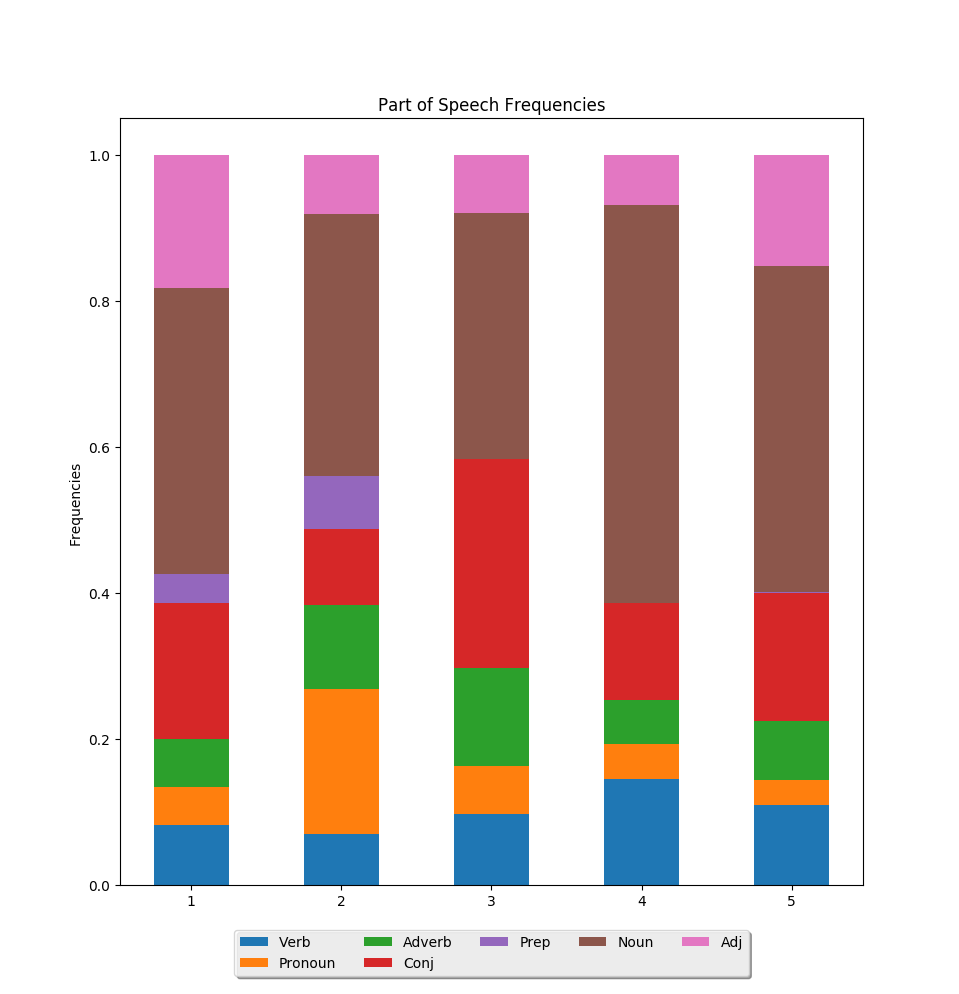
\includegraphics[scale=0.6]{../src/results/parts_of_speech_5}
\end{center}

For the model of 5 hidden states, moderate specialization has occured. In particular, smaller categories such as prepositions and adverbs have significant variance between states. Nouns, however, have similar frequencies across states.

\begin{center}
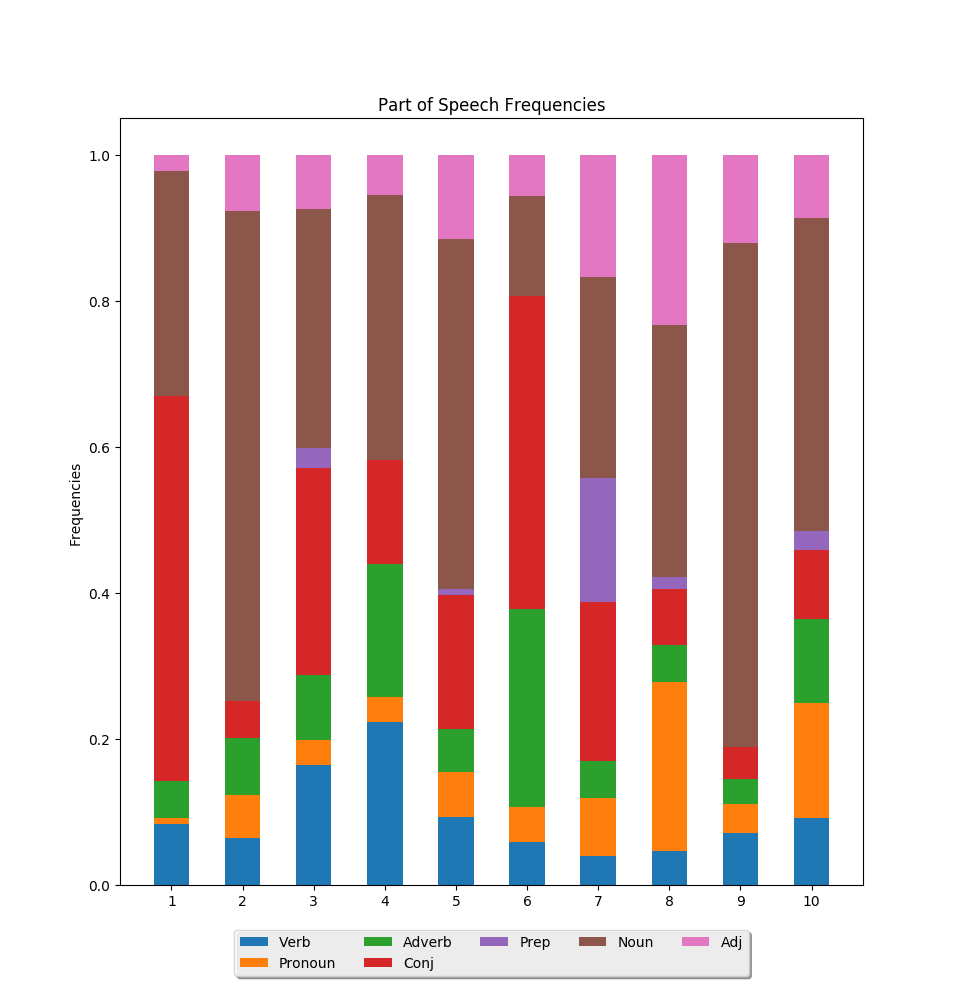
\includegraphics[scale=0.6]{../src/results/parts_of_speech_10}
\end{center}

For the model of 10 hidden states, significant specialization has occured for all parts of speech.

\begin{center}
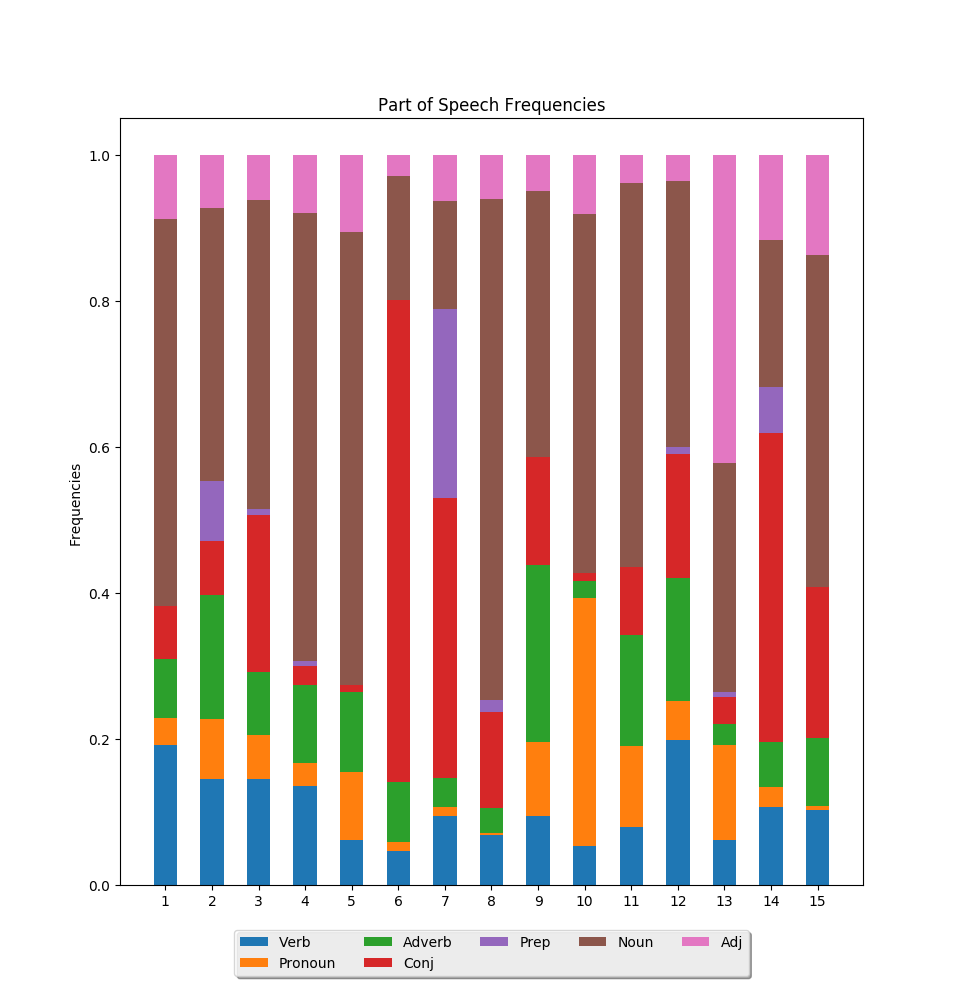
\includegraphics[scale=0.6]{../src/results/parts_of_speech_15}
\end{center}

For the model of 15 hidden states, massive specialization has occured. In particular, prepositions exist almost solely in state 7.

\pagebreak
\section{Appendix C - Syllable Counts}
We trained 3 models, one each of 5, 10, and 15 hidden states. We analyzed how often each state in each model emitted words of different syllabic lengths. We found that, while there were differences between states, they were not as prominent as differences between the frequencies with which states emitted different parts of speech. As a result, it appears more likely that differences in syllable count frequencies are a side effect of the models learning other factors. Note that the data include words with 0 syllables; this is an error on the part of the publicly available code used to count syllables, and in effect represents a reasonable estimate for the error this data. Graphs were generated with Matplotlib.

\begin{center}
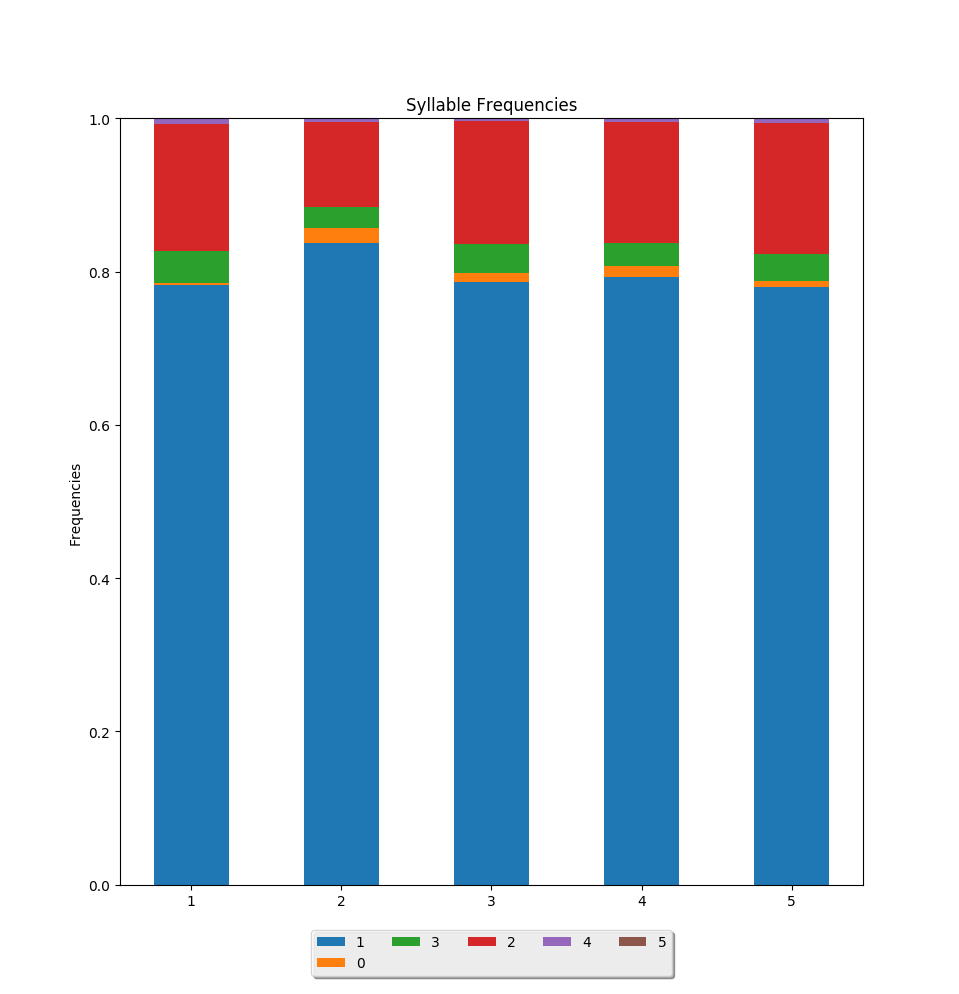
\includegraphics[scale=0.5]{../src/results/syllables_5}
\end{center}

Syllable frequencies for the model of 5 hidden states. Note the lack of variation between states.

\begin{center}
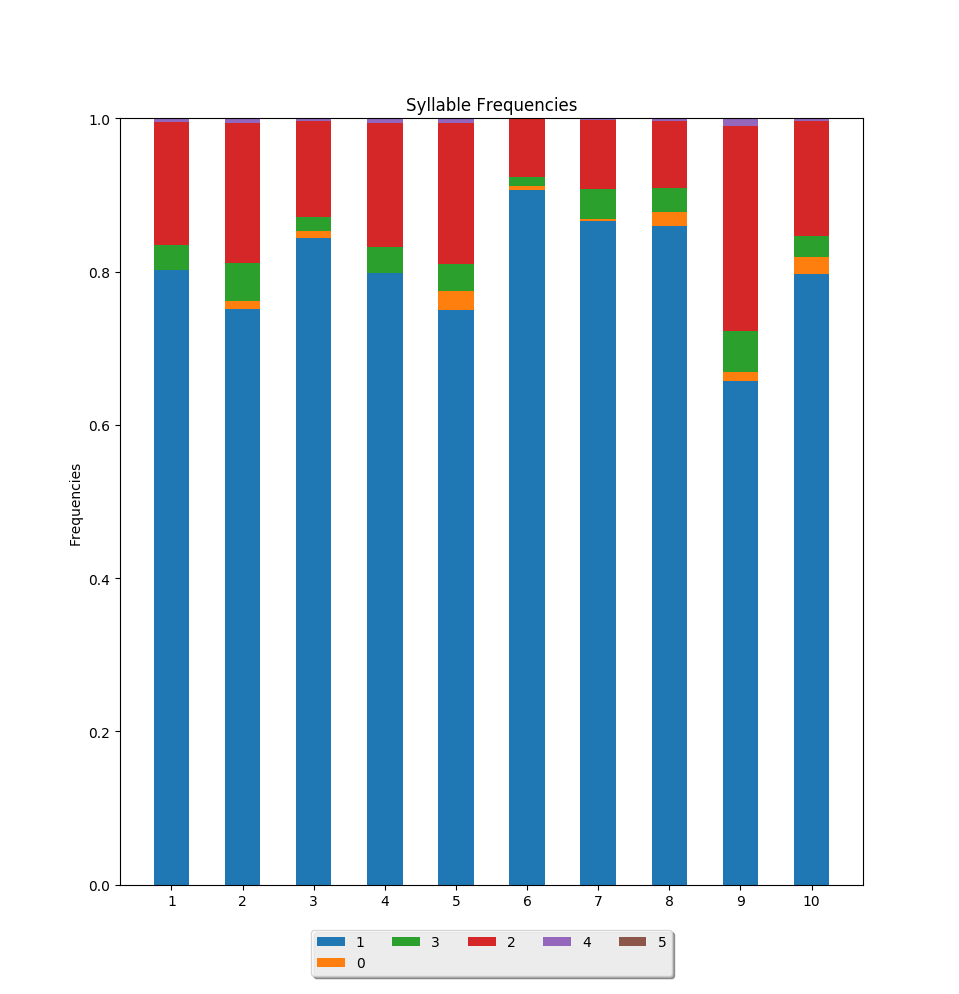
\includegraphics[scale=0.6]{../src/results/syllables_10}
\end{center}

Syllable frequencies for the model of 10 hidden states. This model demonstrates more variance than the model of 5 states, although this is likely an artifact of the model learning other factors (namely, parts of speech).

\begin{center}
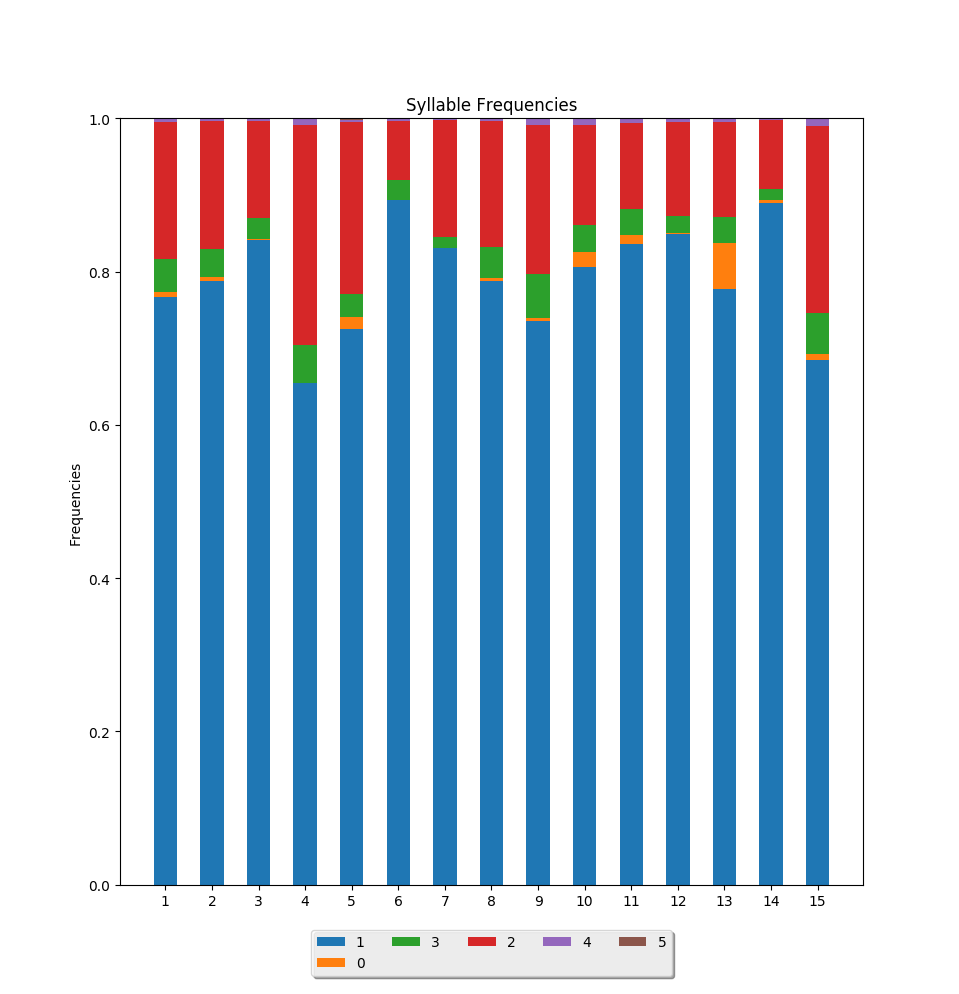
\includegraphics[scale=0.6]{../src/results/syllables_15}
\end{center}

Syllable frequencies for the model of 15 hidden states. As in the model of 10 states, the differences in this data are most likely a side effect of the model learning parts of speech.

\pagebreak
\section{Appendix D - Transition Frequencies}
We visualize the transition frequencies between various states. This information does not explicitly give information about the underlying meaning of states, and is presented here both for completeness and because it is used in visualizing the network of the HMMs.

\begin{center}
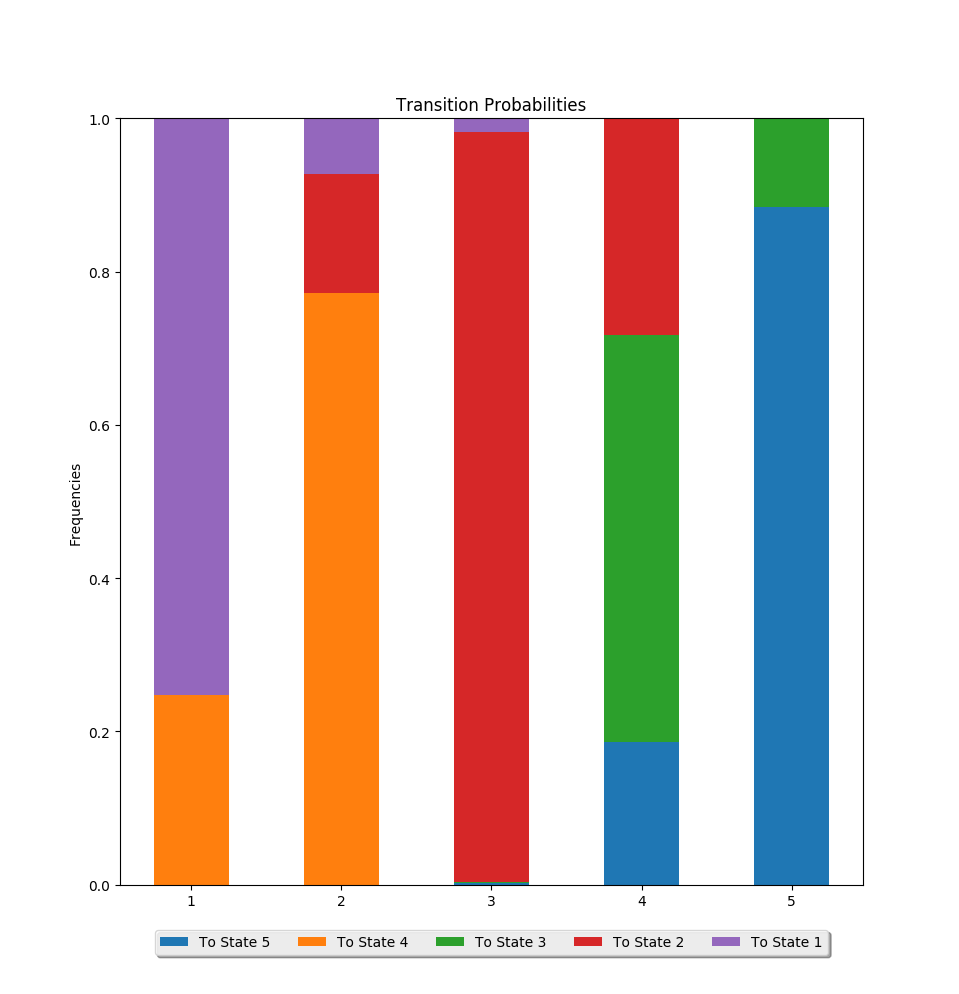
\includegraphics[scale=0.6]{../src/results/transitions_5}
\end{center}

Transition frequencies for the model of 5 hidden states.

\begin{center}
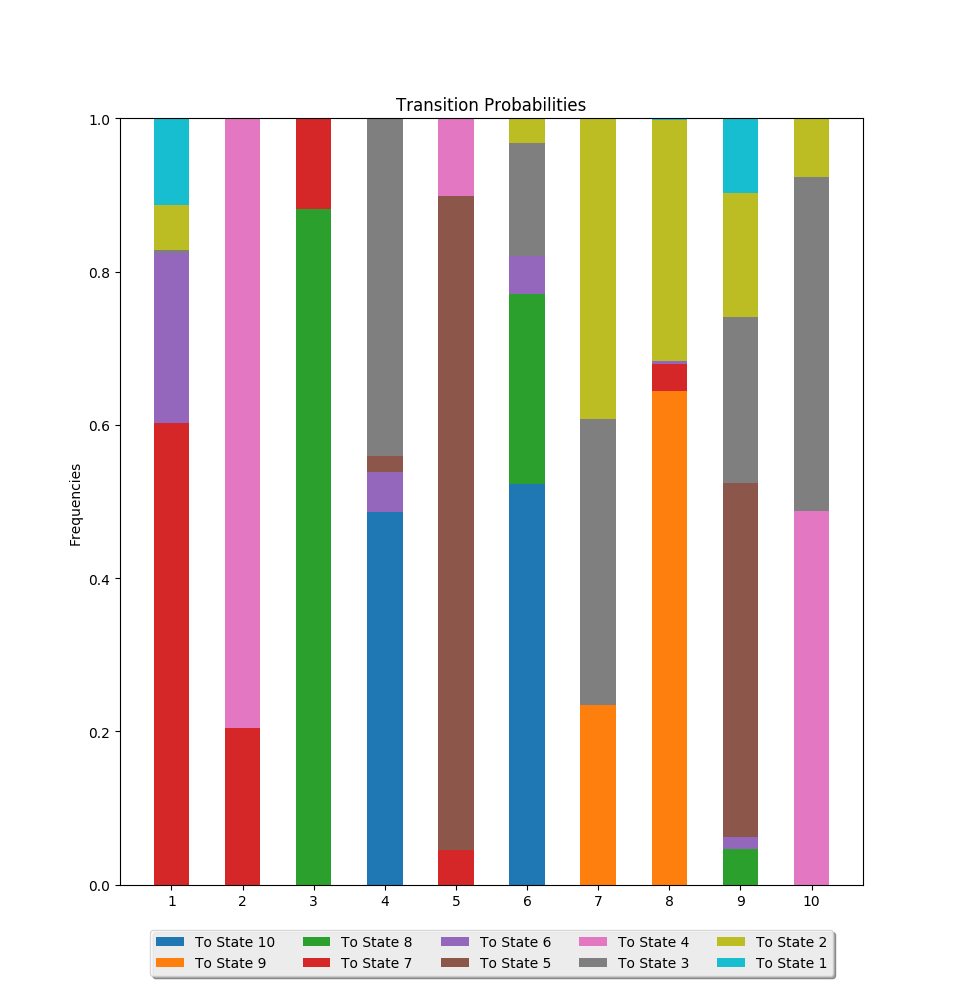
\includegraphics[scale=0.6]{../src/results/transitions_10}
\end{center}

Transition frequencies for the model of 10 hidden states.

\begin{center}
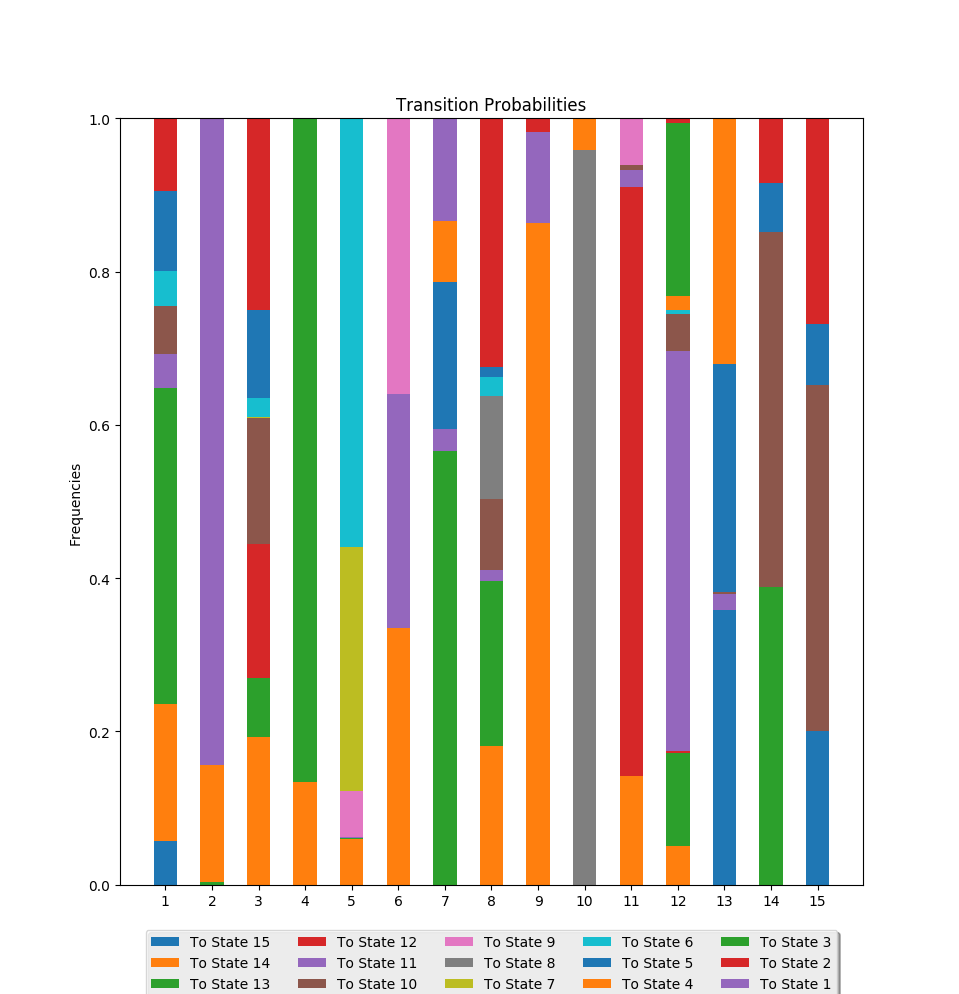
\includegraphics[scale=0.6]{../src/results/transitions_15}
\end{center}

Transition frequencies for the model of 15 hidden states.

\pagebreak
\section{Appendix E - HMM Networks}
We visualize the entire HMM as a network for each model. Each state shows parts of speech that it represents at an unusually high rate (mean + 0.5*std), or (if no part of speech is emitted that frequently) the part of speech that it emits at the highest rate above the mean. Directed edges are added between states when the transition probability is higher than the mean. Given our conclusion that the model learns parts of speech primarily, this provides a visualization of the main parameters learned by our model. Note that the shown parts of speech are those represented disproportionately for the state; this does not mean that the state predominately emits those parts of speech, only that it emits them at an unusually high rate.

\begin{center}
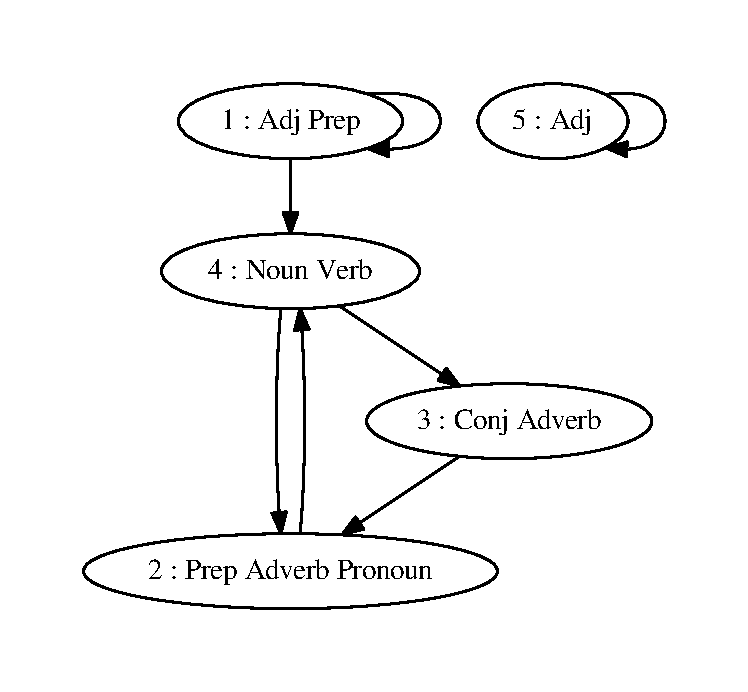
\includegraphics[scale=0.6]{../src/results/graph_5}
\end{center}

Network model for the 5 state HMM. Note the emergence of rudimentary grammatical structure.

\begin{center}
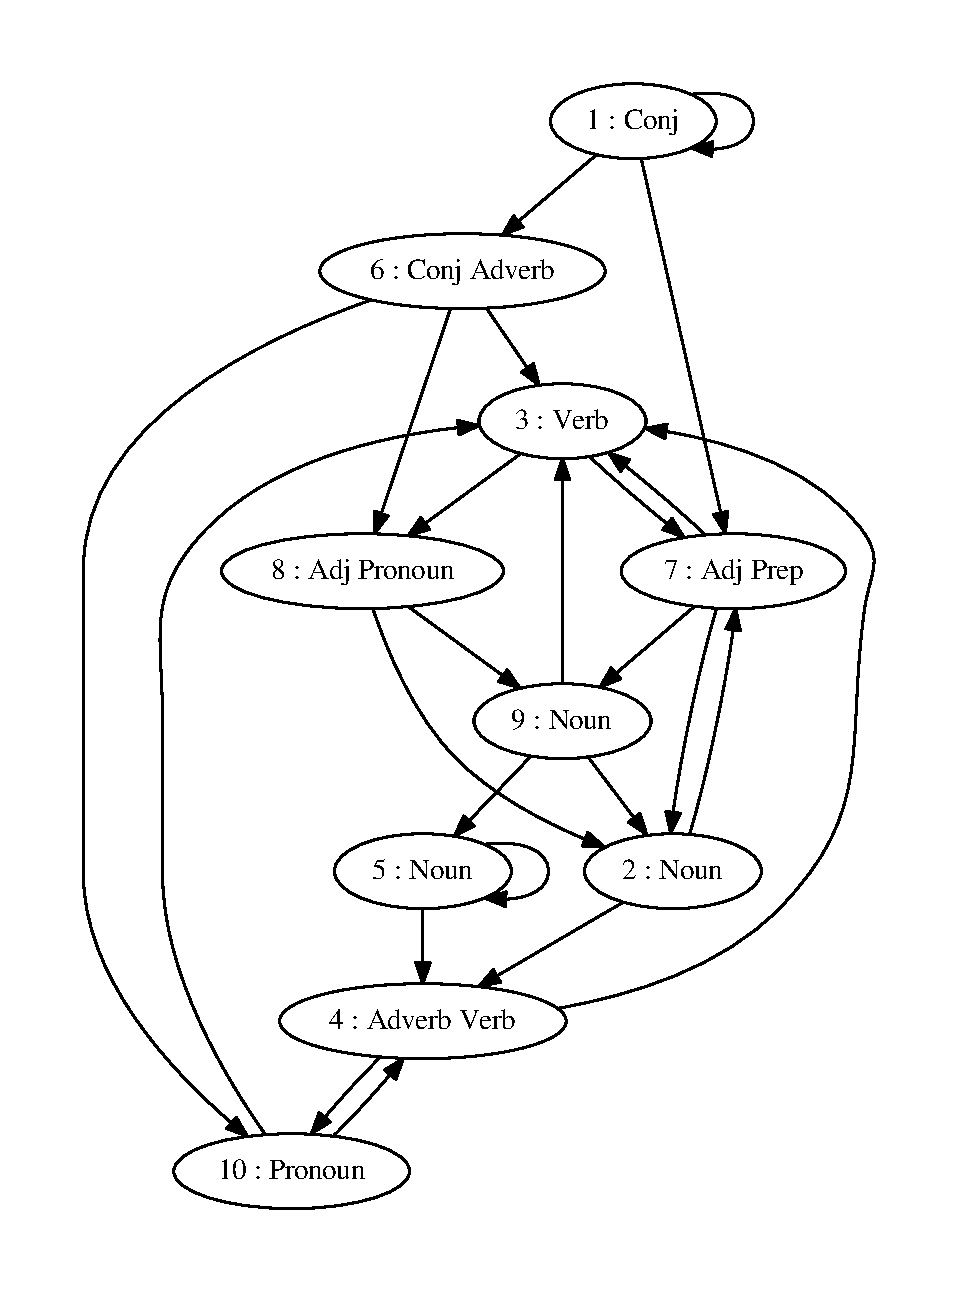
\includegraphics[scale=0.6]{../src/results/graph_10}
\end{center}

Network model for the 10 state HMM. Note the formation of `hubs' at states 2, 3, and 7. Further note the increased grammatical structure evident in the transitions (i.e., Noun states linking to Verb states, Adverbs to Verbs, etc.).

\begin{center}
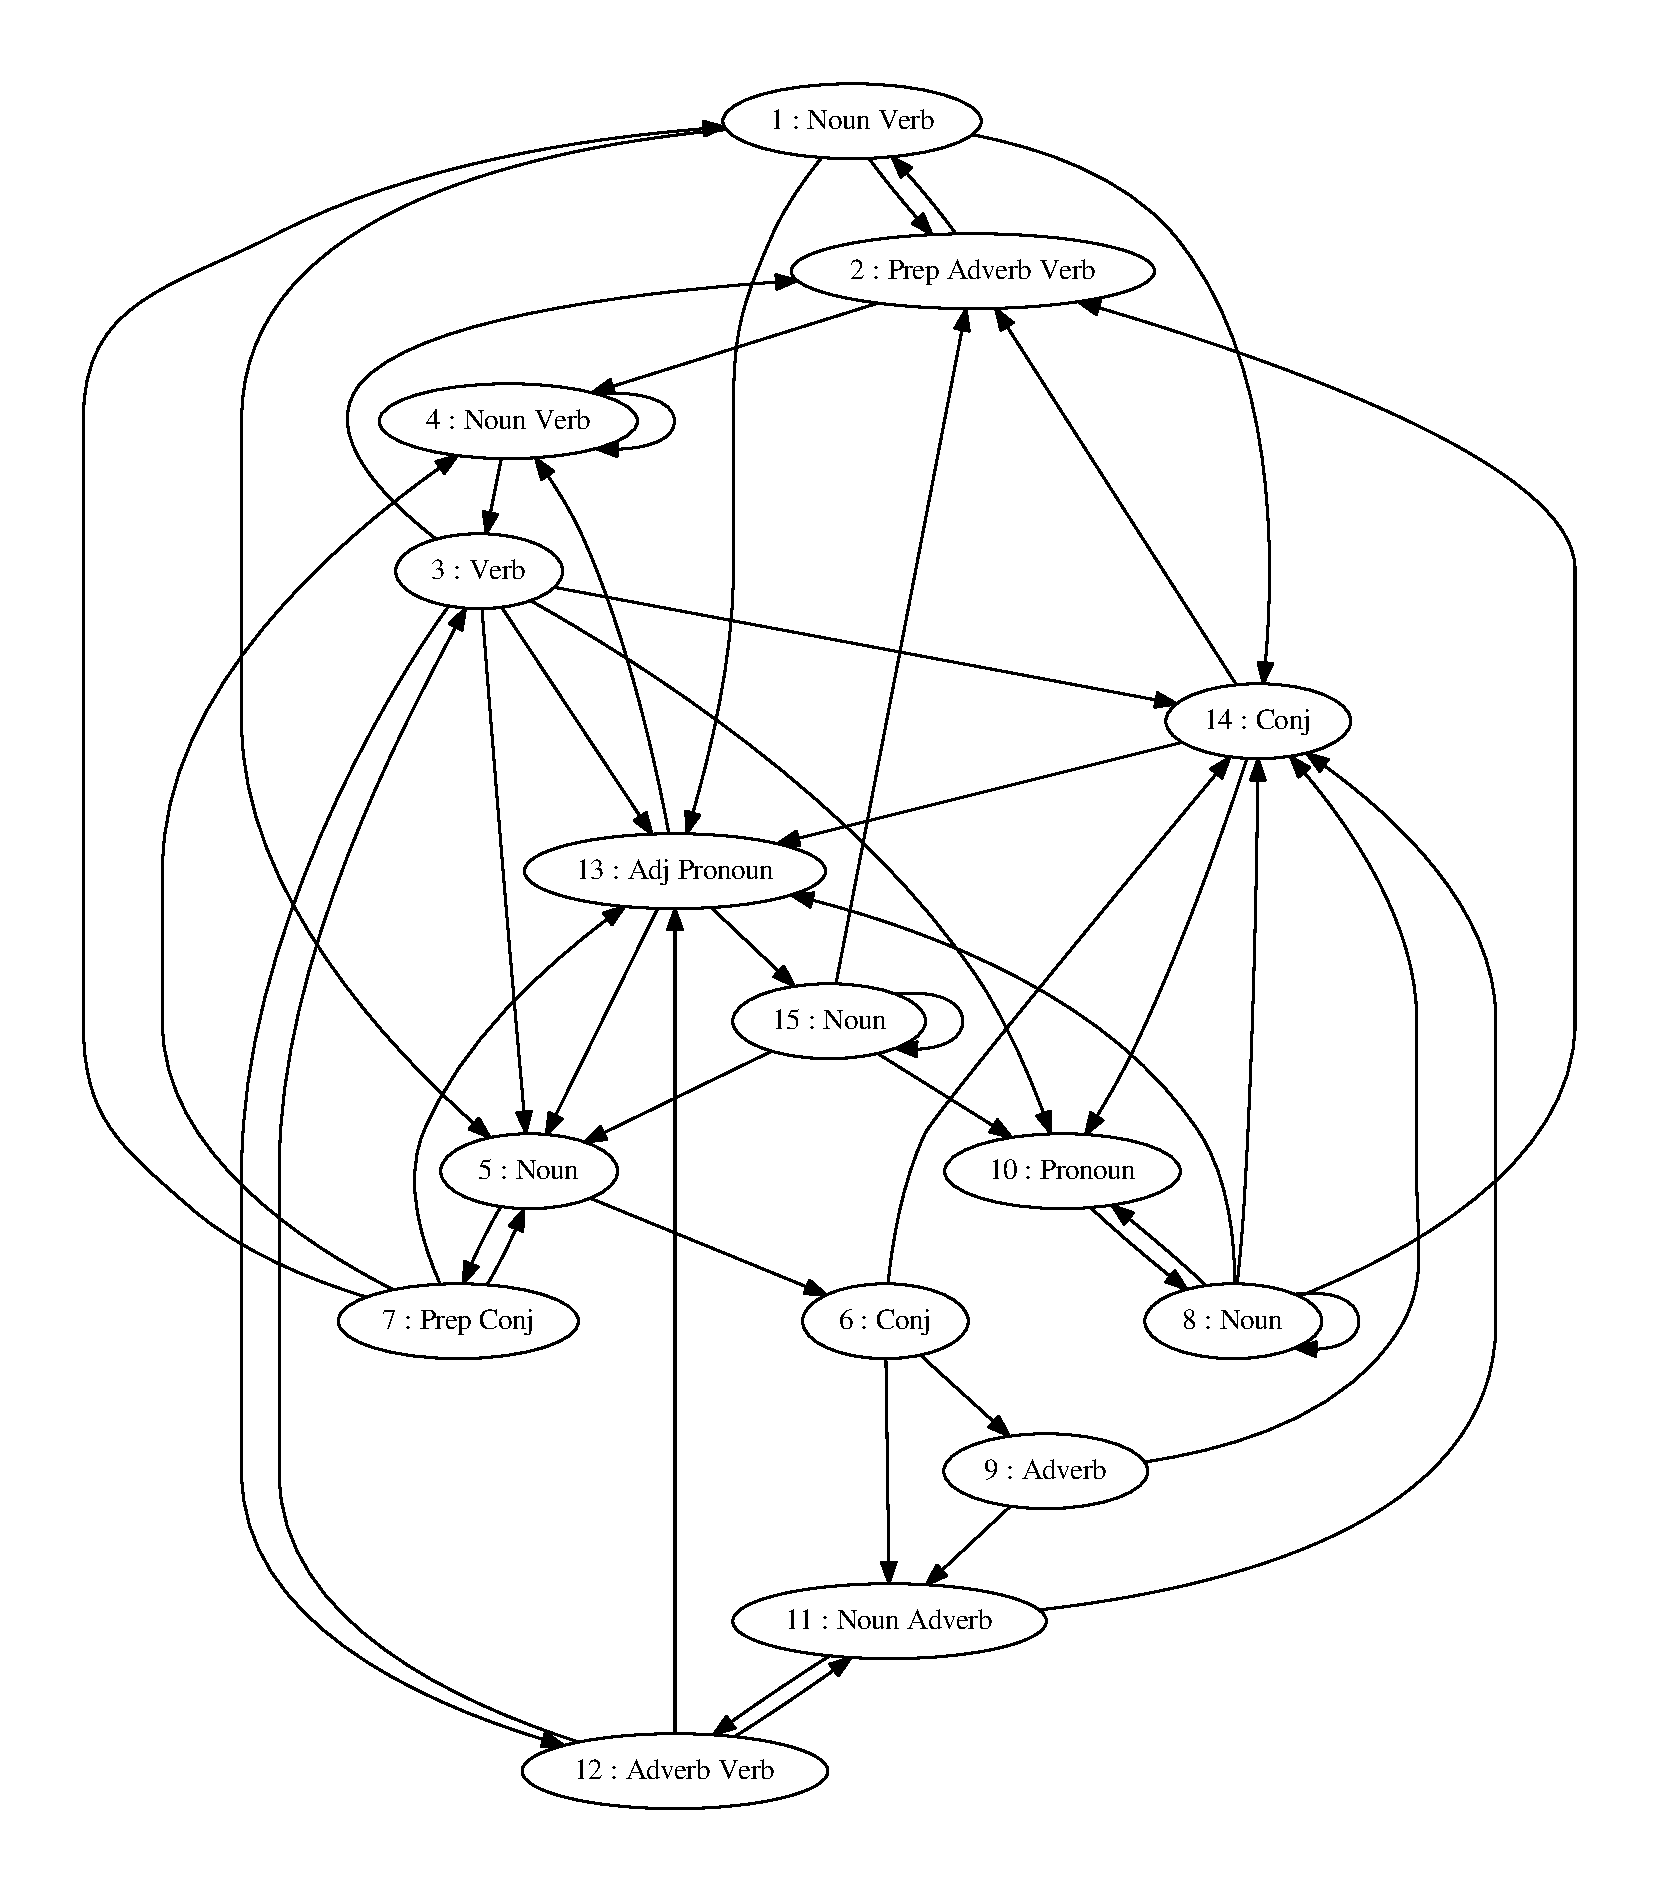
\includegraphics[scale=0.5]{../src/results/graph_15}
\end{center}

Network model for the 15 state HMM. Note the increasing formation of hubs, particularly at states 13 and 14. This is likely a result of the high emission rates of adjectives and conjunctions in 13 and 14, respectively (see Appendix B).

\end{document}